 \documentclass[a4paper,12pt]{article} 
\usepackage[T2A]{fontenc}			
\usepackage[utf8]{inputenc}			
\usepackage[english,russian]{babel}	
\usepackage{amsmath,amsfonts,amssymb,amsthm,mathrsfs,mathtools} 
\usepackage[colorlinks, linkcolor = purple, citecolor = purple]{hyperref}
\usepackage{xcolor}
\usepackage{xpatch}
\usepackage{marvosym}
\usepackage{cancel}
\usepackage{floatrow}
\usepackage{commath}
\usepackage{upgreek}
\usepackage{lipsum}
\usepackage{mhchem}
\usepackage{chemfig}
\usepackage{multirow}
\usepackage{tikz}
\usepackage{titletoc}
\usepackage{pgfplots}
\usepackage{wrapfig}
\usepackage{chngcntr}
\usepackage{makecell}
\usepackage{stackengine,graphicx}
\usepackage{cmap}
\usepackage{indentfirst}
\usepackage{tocloft}
\usepackage{setspace}
\usepackage{titlesec}
\usepackage{soul}
\usepackage[stable]{footmisc}
\usepackage{tocloft}
\usetikzlibrary{positioning}
\usepackage{caption}
\usepackage{subfig}
\pgfplotsset{width=10cm,compat=1.9}
\tikzset{>=stealth}
\usepackage[left=2cm,right=2cm,top=2cm,bottom=3cm,bindingoffset=0cm]{geometry}
%\DeclareMathOperator*{\esssup}{ess\,sup}
\DeclareMathOperator*{\tr}{tr}
\DeclareMathOperator*{\Ker}{Ker}
\DeclareMathOperator*{\Rea}{Re}
\DeclareMathOperator*{\Ima}{Im}
\DeclareFontEncoding{LS2}{}{\noaccents@}
\DeclareFontSubstitution{LS2}{stix}{m}{n}
\DeclareSymbolFont{arrows3}{LS2}{stixtt}{m}{n}
\DeclareMathSymbol{\squareulblack}{\mathord}{arrows3}{"88}
\date{\vspace{-10pt}}
\author{Дорогинин Д.В. Б02-825бф\\
Матвеев Г.А. Б02-824бф}
\title{\textbf{Электронный парамагнитный резонанс.}}


\theoremstyle{definition}
\newtheorem*{definition}{Определение}
\newtheorem{statement}{Предложение}
\newtheorem{lemma}{Лемма}
\newtheorem{theorem}{Теорема}
\newtheorem*{theorem*}{Теорема}
\newtheorem*{corollary}{Следствие}
\newtheorem*{example}{Пример}
\setcounter{tocdepth}{2}
%\renewcommand\cftsecafterpnum{\vspace{-pt}}
%\renewcommand\cftsecafterpnum{\vspace{1pt}}
\newcommand*{\eqdef}{\mathop{\overset{\mathrm{def}}{\resizebox{\widthof{\ensuremath{\mathop{\overset{\mathrm{def}}{=}}}}}{\heightof{=}}{=}}}}
\renewcommand\qedsymbol{$\squareulblack$}
\renewcommand{\cftsecleader}{\cftdotfill{\cftdotsep}}
\newfloatcommand{capbtabbox}{table}[][\FBwidth]
\newcommand{\HH}{\mathcal{H}}
\newcommand{\DD}{\mathcal{D}}
\newcommand{\LL}{\mathcal{L}}
\newcommand{\AAA}{\mathscr{A}}
\newcommand{\SpA}{\mathcal{A}}
\newcommand{\EE}{\mathcal{E}}
\newcommand{\suml}{\sum\limits_{n=1}^\infty}
\newcommand{\sumlN}{\sum\limits_{n=1}^N}
\newcommand{\sumo}{\sum\limits_{n=0}^\infty}
\newcommand{\sumoN}{\sum\limits_{n=0}^N}
\renewcommand\cftsecfont{\normalsize}
\renewcommand\cftsubsecfont{\normalsize}
\titleformat{\section}
  {\normalfont\fontsize{16}{16}\bfseries}{\thesection}{1em}{}
\def\rlwd{.5pt}
\def\crossy{\kern.5pt\def\stacktype{L}%
 \stackon[0.65ex]{%
  \stackon[1.4ex]{%
    \stackon[1.1ex]{\rule{\rlwd}{1.8ex}}{\rule{1.4ex}{\rlwd}}%
  }{\rule{0.8ex}{\rlwd}}%
 }{\rotatebox{-20}{\rule{0.8ex}{\rlwd}}}%
\kern1pt}



\newcommand{\angstrom}{\mbox{\normalfont\AA}}


\begin{document}
\begin{titlepage}
	\begin{center}
		\large 	Московский физико-технический институт \\
		(национальный исследовательский университет) \\
		Факультет общей и прикладной физики \\
		\vspace{0.2cm}
		
		\vspace{4.5cm}
		Лабораторная работа №6.10.4  \\ \vspace{0.2cm}
		\large (Основы современной физики) \\ \vspace{0.2cm}
		\LARGE \textbf{ Магнитный момент лёгких ядер }
	\end{center}
	\vspace{2.3cm} \large
	
	\begin{center}
		Работу выполнил: \\
		Дорогинин Демид,
		группа Б02-825
		\vspace{10mm}			
	\end{center}
		
	\begin{center} \vspace{60mm}
		г. Долгопрудный \\
		2021 год
	\end{center}
\end{titlepage}


\stepcounter{page}
\section*{Аннотация}
В работе исследуется ядерный магнитный резонанс, наблюдается сигнал ЯМР от ядер водорода, опрееляется $g$-фактор для ядер фтора, наблюдается насыщение ядерного магнитного резонанса.
\section*{Теория}
Рассмотрим ядро с магнитным моментом $\boldsymbol{\mu}$ во внешнем поле с индукцией $\mathbf{B}$. Взаимодействие магнитного диполя с внешним полем приводит к появлению дополнительной энергии 
\[
E = -(\boldsymbol{\mu},\mathbf{B}).
\]
Вектор $\boldsymbol{\mu}$ ориентирован по направлению полного момента количества движения $\mathbf{M}$:
\[
\boldsymbol{\mu} = \gamma \mathbf{M},
\]
где $\gamma$ -- гиромагнитное соотношение. Вводя ядерный $g$-фактор, значение которого постоянно на одном уровне,
\[
g = \dfrac{\hbar}{\mu_\text{я}}\gamma,
\]
перепишем в виде
\[
\boldsymbol{\mu} = \dfrac{\mu_\text{я}}{\hbar}g\mathbf{M}.
\]
Квадрат вектора $\mathbf{M}$ и его проекция определяются формулами
\[
\mathbf{M}^2 = \hbar^2 I(I+1),~M_z = m\hbar,
\]
гдн $I$, целое или полуцелое число, -- спин ядра, а $m$ -- целое число, по модулю не превосходящее $I$. Тогда, проектируя $\mathbf{M}$ и $\boldsymbol{\mu}$ на направление вектора $B$, получим
\[
\mu_B = \dfrac{\mu_\text{я}}{\hbar}g M_B = \mu_\text{я} g m.
\]
Таким образом, разница между расщепившимися уровнями энергии будет
\[
\Delta E = B\Delta \mu_B = B \mu_\text{я} g.
\]
Между компонентами расщепившегося уровня могут происходить электромагнитные перезоды. Переходы с нижних компонент на верхние требуют затрат энергии и происходят лишь под действием внешнего высокочастотного поля. Энергия квантов, вызывающих электромагнитные переходы, точно определена, стало быть явление носит резонансный характер. Соответствующая частота 
\begin{equation}
\omega = \dfrac{\Delta E}{\hbar} = \dfrac{\mu_\text{я}}{\hbar}Bg.
\end{equation}
Возбуждение переходов между компонентами расщепившегося ядерного уровня носит название \textit{ядерного магнитного резонанса}.
\section*{Установка}
\begin{figure}[h]
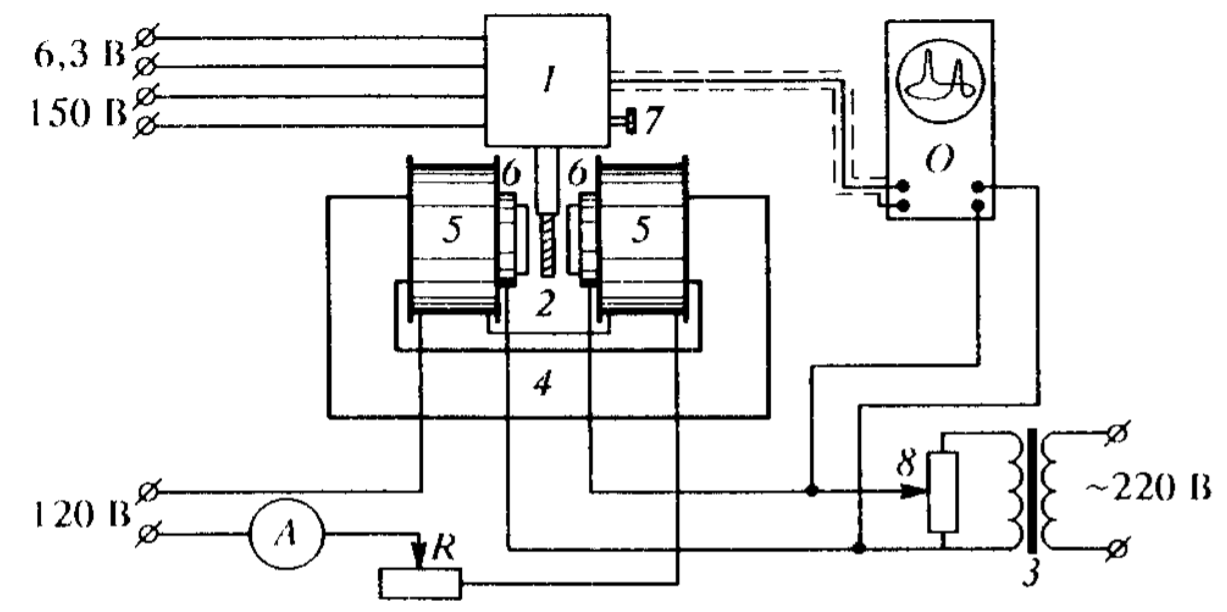
\includegraphics[width=0.7\textwidth]{1.png}
\centering
\caption{Схема установки.}
\end{figure}
На Рис. 1 изображена схема установки. Образец 2 помещён внутрь катушки, входящей в состав генератора. Генератор представляет собой часть индикаторной установки 1, магнитное поле в образце создаётся с помощью электромагнита 4. Основное магнитное поле создаётся с помощью катушек 5, питаемых постоянным током. Величина тока регулируется реостатом $R$ и измеряется амперметром $A$. Небольшое дополнительное поле возбуждается модулирующими катушками 6, присоединёнными к сети переменного тока через трансформатор 3. Напряжение на катушках регулируется потенциометром 8.\\
Основной частью установки является генератор слабых колебаний. Он представлет собой усилитель с положительной обратной связью, благодаря которой поддерживается непрерывная генерация. Катушка с образцом и находящийся в ящике 1 конденсатор переменной ёмкости образуют сеточный контур генератора. Ёмкость конденсатора можно менять, поворачивая лимб 7. При наступлении ЯМР поглощение энергии в образце увеличивается, добротность сеточного контура падает и амплитуда генерации уменьшается. Высокочастотный сигнал с генератора усиливается и детектируется.\\
Детектирование сигнала ЯМР осуществляется с помощью промышленного прибора. Модуляция магнитного поля осуществляется с помощью небольшой катушки, частота модуляции $\approx$ 50 Гц. В зазоре электромагнита устанавливается холловский измеритель магнитного поля, а измерения ЯМР проводятся на резине (измеряется ЯМР на протонах), тефлоне (в состав входит фтор) и тяжелой воде.\\
Сигнал ядерного магнитного резонанса наблюдается на экране осциллографа. На рис. 2 вверху изображен временной ход магнитного поля электромагнита. Как уже отмечалось, постоянная часть поля создается основными, а переменная -- модулируюшими катушками. При правильной настройке установки магнитное поле колеблется около резонансного значения, пересекая его два раза за каждый период изменения тока в модулирующих катушках. Как видно из Рис. 2, время, проходящее между следуюшими друг за другом пересечениями, одинаково при точном равенстве постоянного магнитного поля резонансному значению $B_{0}$ (Рис. 2а) и различается при неточном их соответствии (Рис. 2б) основной составляющей магнитного поля.

\begin{figure}[h]
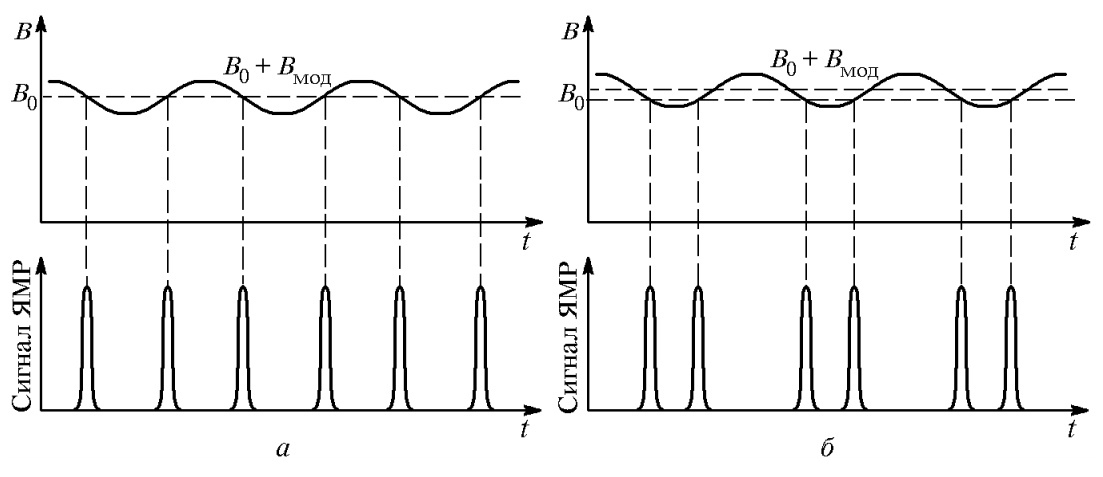
\includegraphics[width=0.85\textwidth]{2}
\centering
\caption{Временная зависимость магнитного поля и сигнала ядерного магнитного резонанса.}
\end{figure}
\section{Выполнение и обработка данных}
Найдём рещонансную частоту $f_{\text{рез}}$ для четырёх различных образцов, после через с помощью детектора Холла определим магнитное поле в щели прибора. Результаты в Таблице 1.
\begin{table}[h!]
\begin{tabular}{|c|c|c|c|c|}
\hline
№ & Образец      & $f_{\text{рез}}$,   МГц & $B_{\text{холл}}$,   мТл & $B_0$, мТл \\ \hline
1 & Резина       & 9.88                        & 229                         & 232.0           \\ \hline
2 & Тефлон       & 9.87                        & 243                         & 231.9           \\ \hline
3 & Вода         & 9.37                        & 227                         & 228.5           \\ \hline
4 & Тяжелая вода & 3.42                        & 521                         & 522.3           \\ \hline
\end{tabular}
\centering
\caption{Результаты измерения постоянного магнитного поля и резонансной частоты.}
\end{table}

Для каждого образца вычислим $g$-фактор и магнитный момент ядра, далее используем ядерный магнетон
$$
\mu_{\text{я}} \approx 5.05 \cdot 10^{-27} \text{ } \frac{\text{Дж}}{\text{Тл}}.
$$

\subsection{Образецы №1 и №3 -- резина и вода (ЯМР на протонах)}

Величина ядерного $g$-фактора для протона определяется по формуле
$$
g_{p}=\frac{h f_{0}}{\mu_{\text{я}} B_{0}}
$$
Так как угловой момент протона определяется только его спином, то по величине $g$-фактора легко рассчитать и магнитный момент
$$
\mu_{p}=g_{\mathrm{p}} \mu_{\text{я}} I=\frac{g_{p}}{2} \mu_{\text{я}}.
$$
В результате вычисленные значения совпали с табличными.
$$
\mu_{p_\text{табл}} = 2.7928 \mu_{\text{я}}.
$$

\subsection{Образец №2 -- тефлон (ЯМР на ядрах фтора)}
Аналогично вычисляется величина $g$-фактора ядра фтора, а затем его магнитный момент. Величина $g$-фактора и магнитного момента близка к значению для протона, так как орбитальное движение протона не вносит вклад в магнитный момент этого ядра, и он определяется только спином протона.

$$
\mu_{\ce{F}_{\text{табл}}} = 2.6285 \mu_{\text{я}}.
$$

\subsection{Образец №4 -- тяжелая вода (ЯМР на дейтронах)}
Здесь измеряется ЯМР на дейтронах. Величина $g$-фактора определяется по аналогичной формуле. 

Спин дейтрона равен 1, поэтому его магнитный момент
\[
\mu_{p}=g_{\mathrm{p}} \mu_{\text{я}} I=g_{p} \mu_{\text{я}} 
\]
При этом табличное значение:
\[
\mu_{\ce{D}_{\text{табл}}}=0.857 \mu_{\text{я}}
\]
Предположим, что основное состояние дейтрона является не чистым S-состоянием, а смесью состояний $\ce{^3S1}$ и $\ce{^3D1}$ (с  $ L=2) .$ Если $P_{\ce{S}}$ и $P_{\ce{D}}$ -- статистические веса этих состояний, то
$$
\mu_{d}=\mu_{n}+\mu_{p}-\frac{3}{2}\left(\mu_{n}+\mu_{p}-\frac{1}{2}\right) P_{\ce{D}}
$$
Отсюда, зная табличные значения магнитных моментов протона и нейтрона и используя
найденное значение магнитного момента дейтрона, найдем $P_{\ce{D}}$:
$$
\mu_{p}=2.792763 \mu_{\text{я}},~\mu_{n}=-1.91315 \mu_{\text{я}} 
$$

$$
P_{\ce{D}}=\frac{2}{3} \frac{\mu_n+\mu_p-\mu_d}{\mu_n+\mu_p-\frac{1}{2}}=(5.0 \pm 1.6) \%
$$


Итоговые реультаты представим в Таблице 2.
\begin{table}[h!]
\begin{tabular}{|c|c|c|c|c|}
\hline
№ & Образец      & $g_{\text{я}}$ & $\sigma_{g_\text{я}}$ & $\mu, \mu_{\text{я}}$ \\ \hline
1 & Резина       & 5.59           & 0.05                  & 2.79                  \\ \hline
2 & Тефлон       & 5.35           & 0.05                  & 2.67                  \\ \hline
3 & Вода         & 5.38           & 0.05                  & 2.69                  \\ \hline
4 & Тяжелая вода & 0.85           & 0.01                  & 0.85                  \\ \hline
\end{tabular}
\centering
\caption{Результаты вычисления $g$-факторов и магнитных моментов ядер.}
\end{table}
\section{Вывод}
В ходе работы были вычислены магнитные моменты протона, дейтрона и ядра фтора на основе измерения их $g$-факторов методом ядерного магнитного резонанса (ЯМР). Полученные данные сравнивались с вычислениями магнитных моментов на основе кварковой модели адронов и одночастичной оболочечной модели ядер.

В результате магнитный момент и $g$-фактор протона хорошо согласуются с табличными значениями, значения магнитного момента и $g$-фактора ядра фтора оказались близки к соответствующим значениям для протона, как и предсказывает теория, для дейтрона проведен расчёт статистического веса состояния $\ce{^3D1}$.

\begin{thebibliography}{9}
\bibitem{laba} 
Игошин Ф.Ф., Самарский Ю.А., Ципенюк Ю.М.
\textit{Лабораторный практикум по общей физики: Учеб. пособие для вузов. Т3. Квантовая физика.}. 
М.: Физматкнига - 2005.
\end{thebibliography}
\end{document}










